\documentclass[conference]{IEEEtran}

\usepackage{cite}
\usepackage{url}
\usepackage{fontawesome5}
\usepackage{multirow}

\ifCLASSINFOpdf
  \usepackage[pdftex]{graphicx}
\else
  \usepackage[dvips]{graphicx}
\fi
\graphicspath{{./img/}}
\DeclareGraphicsExtensions{.pdf,.jpeg,.png,.svg}

% correct bad hyphenation here
\hyphenation{op-tical net-works semi-conduc-tor}


\begin{document}
\title{Hardware and System Specification Command-Line~Interface Tool}
\author{\IEEEauthorblockN{Evan Elias Young}
\IEEEauthorblockA{College of Engineering and Computing\\
Missouri University of Science and Technology\\
Rolla, Missouri 65401--3066\\
Email: eeymrr@umsystem.edu}}
\maketitle

\begin{abstract}
There are many tools available to retrieve system specifications, however many of these lack cross-platform support and machine-readable output.
Many different operating systems include a command-line interface to retrieve some part of the information, however this is often not human-readable.
A single tool which works on every operating system, includes human-readable output, and implements native libraries to quickly retrieve accurate information is necessary.
Working together many different system libraries, formats, data types, and parsing revealed which operating systems include the most legacy code, which operating systems are the most streamlined, and the way in which libraries come together to form a cohesive application.
\end{abstract}
~\\
\begin{IEEEkeywords}
Namespace, WMI (Windows Management Instrumentation), JSON (JavaScript Object Notation)
\end{IEEEkeywords}

\section{Background}
CSpec is a hardware and system specification command-line interface tool, where a user can query
the system for different information regarding hardware and software.
A user will either 'list' the available queries or namespaces, or 'get' a data member or entire namespace of data members.
The output will be delivered in one of several ways: list, compact, value (only), or json, all supporting human-readable numerical values.

With the operating system determined at compile time, the compiler will know which header, source, and template files to include.
This is powerful as it reduces the amount of compiled and included code to only what is necessary.
This also ensures that the code will not fail to build, since each operating system is required to implement the same methods,
where shims can be implemented on a per-system basis.

\section{Implementation}
Both the makefile and the primary header determine which operating system the host is running,
either to link different libraries or to define override functions.
Windows requires several libraries to be built into the distributable, and several libraries to
be linked to provide access to WMI and the registry.

\subsection{Windows}
Windows includes a very archaic method of dealing with strings, oftentimes requiring a separate string macro (BSTR)
which will use wide characters or whichever legacy character your build of Windows supports.
As such, conversion from standard characters to wide characters was included, and static casting was a necessity.

WMI was used for a vast majority of the system information,
and \cite{whims:wmi} was used to wrap the functionality into a class (ensuring safe destruction).
WMI requires a significant amount of setup, and at any point in the process could fail, which is why
wrapping this in a class provided an intuitive endpoint of failure checking and resource freeing on failure.

The registry was another point of data access, and \cite{dicanio:winreg} was used as a guide to set up
access and conversion methods.

\subsection{macOS}
macOS relied on the use of two system specific libraries; sysctl and system profiler.
\cite{aapl:sysctl} was used to configure and research the sysctl utilization within C++ and macOS.
While fairly intuitive, retrieving strings with sysctl required a temporary buffer and trimming on null characters.

System profiler unfortunately has no public-facing C++ headers, and therefore cannot be invoked directly in C++.
As a workaround, running system profiler in bash and capturing the output into a buffer was used.
In addition to system profiler's innate slowness (I am ignorant as to why),
running a shell command and streaming into a buffer increases the runtime.

\subsection{Linux}

\section{Semantics}
Semantics describe the methodology behind design choices which do not effect the functionality of the project.

\subsection{Organization}
Within each namespace, there are different queries a user can make;
Separating these queries into folders identified by the namespace was a logical conclusion.
Each namespace folder contains a single header for function headers, namespace types, header inclusions, etc.,
a source file for collecting queries, and a source file for JSON conversion.

A shared namespace is used for general project utilities, such that the amount of header-source files are reduced and
incremental patching of source files. Of importance is that this also allow for operating system specific
headers and functionality to be included at compile time, with further scoped namespaces.

\subsection{Templates}
In standard C++, convention is to include templated methods and classes in either a header file (.h) or header-source file (.hpp).
As these two file extensions are based on the notion of being a header, it can obfuscate whether or not the file is compiled, or built into a source file.
Header files are neither compiled nor built-in, whereas header-source files are not compiled but built-in to a source file.
This removes the ability for make and cmake to determine whether or not the source file has been updated, which is where a template file (.tpp) applies.

Template files will be included at the end of a header (.h) file, and will therefore always mark a source file as updated.
Since the source file includes the header file prior to compilation, it will notice a change and rebuild accordingly.

\section{Libraries}

\subsection{JSON for Modern C++}
JSON parsing was desired as it is easily machine readable and very portable, therefore some implementation of JSON was required.
\textit{JSON for Modern C++} was chosen as a single-header option, written for C++17 it includes very modern features and encourages the use of these quite well.
In addition to modern features, the structuring and destructing is simple to implement and very efficient.

\begin{figure}[!t]
    \centering
    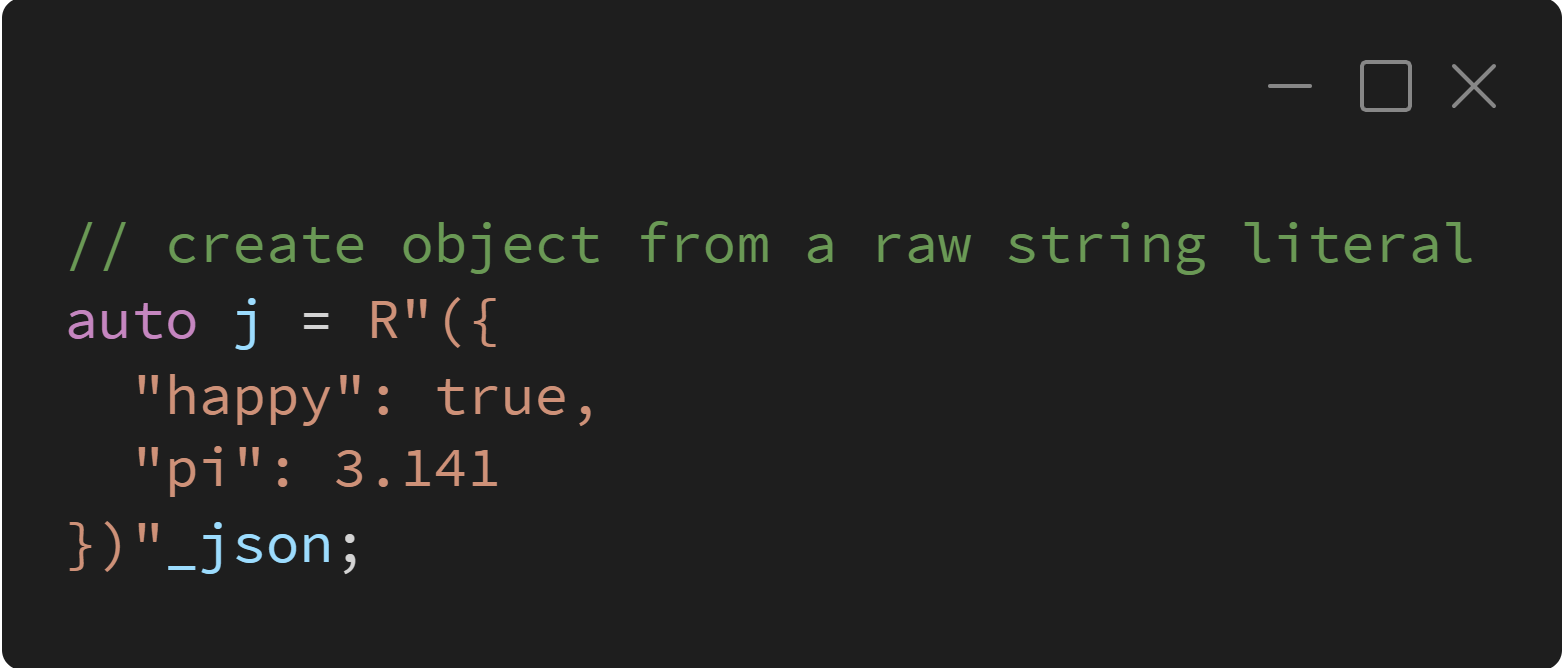
\includegraphics[width=\linewidth]{fig-json}
    \caption{Declaration of simple JSON object through the use of raw string literal suffixes.}
    \label{fig-json}
\end{figure}

\subsection{Argument Parser for Modern C++}
For a command-line interface, argument parsing was necessary to differentiate queries, listings, and selection.
\textit{Argument Parser for Modern C++} was chosen as a single-header option, written for C++17 it includes very modern features and encourages the use of these quite well.
In addition to modern features, the implementation and usage is very similar to python and is quite efficient too.

\begin{figure}[!t]
    \centering
    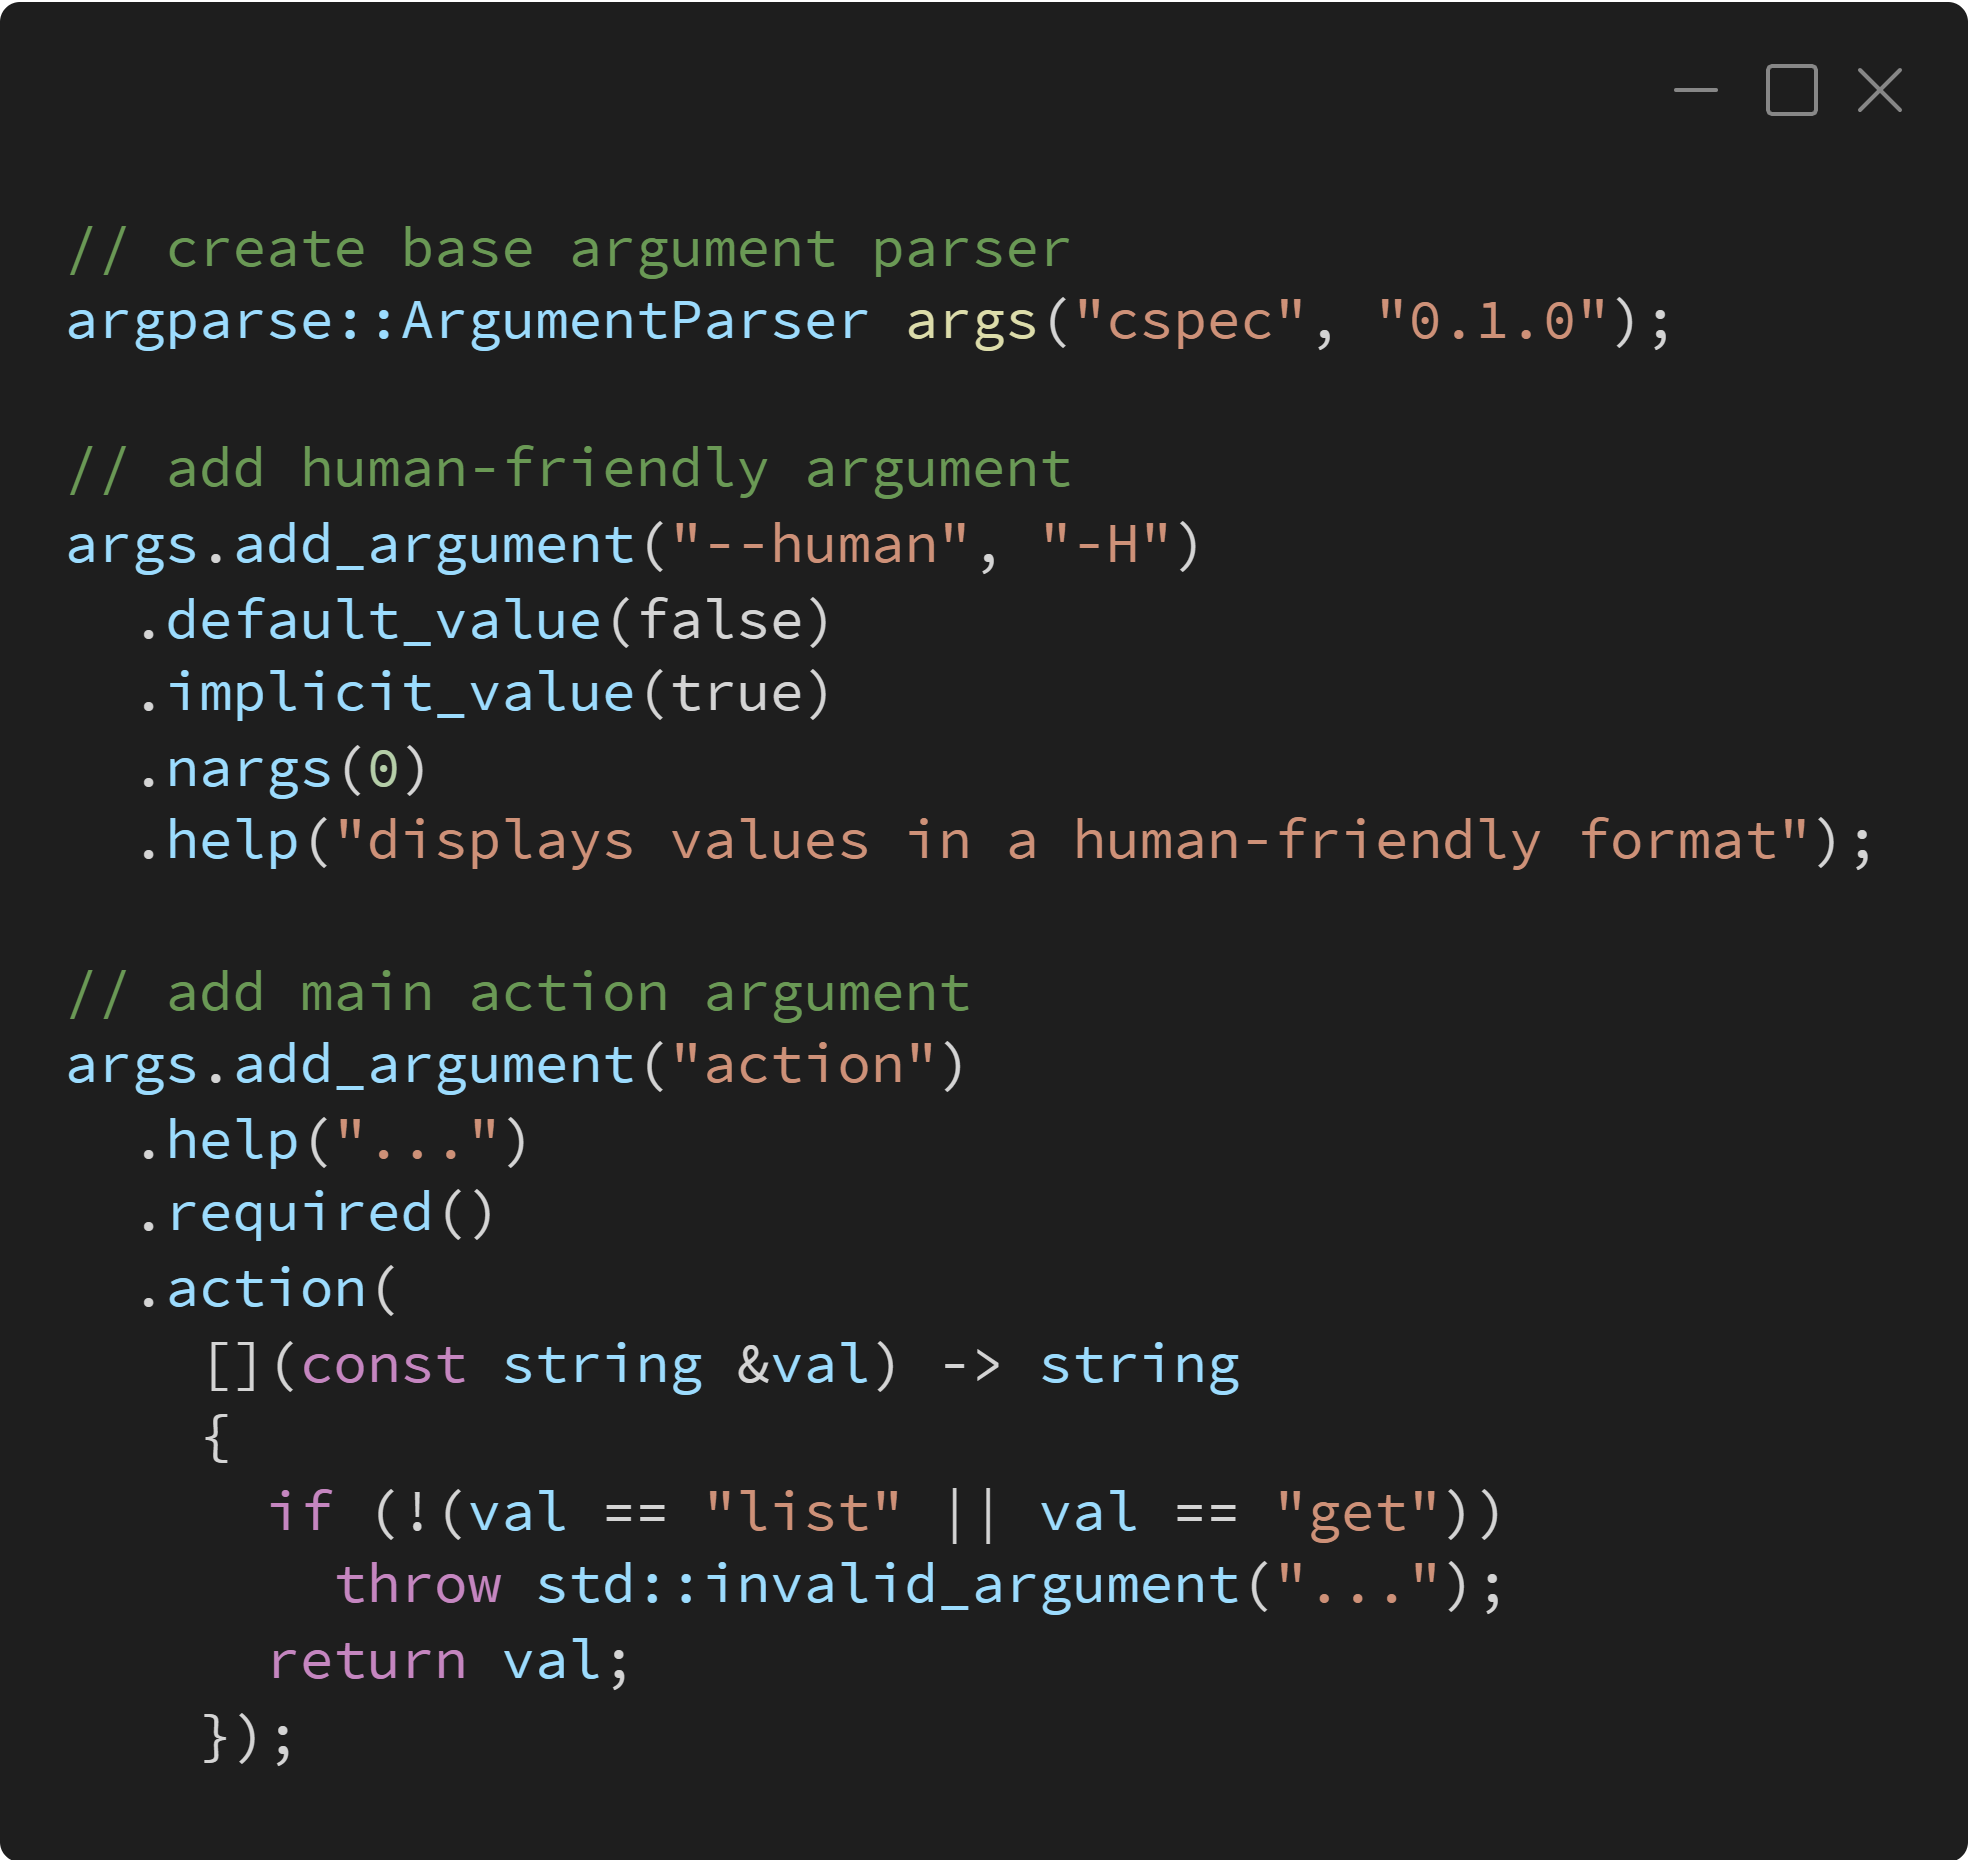
\includegraphics[width=\linewidth]{fig-argparse}
    \caption{Declaration of argument parser object with one optional flag and one positional action.}
    \label{fig-argparse}
\end{figure}

\section{Conclusion}
\begin{table}
    \caption{Project Build Information}
    \label{table_build_times}
    \centering
    \begin{tabular}{|c||c|c|c|}
        \hline
        OS & Threads & Build Time [s] & Build Size [MB] \\
        \hline
        \hline
        Windows 11 & 24 & 28.98 & 1.7351 \\
        \hline
        macOS 12.1 $\beta$1 & 10 & 24.10 & 1.2134 \\
        \hline
        Ubuntu 21.10 & 3 & 92.46 & 1.3135 \\
        \hline
    \end{tabular}
\end{table}
\begin{table}
    \caption{OS Support Information}
    \label{table_support}
    \centering
    \begin{tabular}{|c||c|c|c|}
        \hline
        Query & Windows & macOS & Linux \\
        \hline
        \hline
        cpu & \multicolumn{3}{c|}{\faCheck} \\
        \hline
        filesystem & \multicolumn{3}{c|}{\faCheck} \\
        \hline
        gpu & \multicolumn{2}{c|}{\faCheck} & \faPlus \\
        \hline
        gpu.bus & \multicolumn{2}{c|}{\faCheck} & \faMinus \\
        \hline
        gpu.dynamic & \multicolumn{2}{c|}{\faCheck} & \faMinus \\
        \hline
        memory & \multicolumn{2}{c|}{\faCheck} & \faMinus \\
        \hline
        memory.manufacturer & \faTimes & \faCheck & \faMinus \\
        \hline
        memory.voltage & \faCheck & \faTimes & \faMinus \\
        \hline
        system & \multicolumn{3}{c|}{\faCheck} \\
        \hline
    \end{tabular}
\end{table}
\begin{table}
    \caption{Output Style Examples}
    \label{table_format}
    \centering
    \begin{tabular}{|c||c|c|c|c|}
        \hline
        Format & List & Compact & Value & JSON \\
        \hline
        \multirow{2}{*}{Default}& ... & \multirow{2}{*}{...=2000} & \multirow{2}{*}{2000} & \multirow{2}{*}{\{"...": 2000\}} \\
        &2000&&&\\
        \hline
        \multirow{2}{*}{Human}& ... & \multirow{2}{*}{...=2 KB} & \multirow{2}{*}{2 KB} & \multirow{2}{*}{\{"...": "2 KB"\}} \\
        &2 KB&&&\\
        \hline
    \end{tabular}
\end{table}

\subsection{Product}
Most queries are supported on every operating system, Table \ref{table_support} details which queries are
supported (\faCheck), not supported (\faTimes), partially supported (\faPlus), and pending implementation (\faMinus)
on each operating system.

Time constraints restriced my ability to fully implement Linux support regarding the gpu and memory namespaces,
while system contraints restricted my ability to fully implement the Windows and macOS namespace.

All different styles of formatting output were implemented successfully, Table

\subsection{Knowledge}
During the course of the project, I learned how to use git submodules, how to use external user-level libraries (see \cite{lohmann:json} and \cite{pranav:argparse}),
and how to interface with lower level system libraries (see \cite{whims:wmi} and \cite{dicanio:winreg}).

Segmentation of large amounts of operating system-dependent source code was an additional topic with which I was unfamiliar;
this required different syntax in my makefile which supported recursing through directories of source code.

\section*{Acknowledgment}

I would like to thank Niels Lohmann et. al. for their contributions to \textit{JSON for Modern C++},
and Pranav et. al. for their contributions to \textit{argparse}.

\newpage

\begin{thebibliography}{2}

\bibitem{whims:wmi}
S.~Whims, V.~Kents, et.~al., \textit{Example: Getting WMI Data from the Local Computer}, Microsoft, Jan. 7, 2021. Accessed: Nov. 30, 2021. [Online]. Available: \url{https://docs.microsoft.com/en-us/windows/win32/wmisdk/example--getting-wmi-data-from-the-local-computer}.

\bibitem{dicanio:winreg}
G.~Dicanio, "Use Modern C++ to Access the Windows Registry" \textit{MSDN}, vol. 32, no. 5, May. 2017. Accessed: Nov. 30, 2021. [Online]. Available: \url{https://docs.microsoft.com/en-us/archive/msdn-magazine/2017/may/c-use-modern-c-to-access-the-windows-registry}.

\bibitem{pranav:argparse}
P.~Ranav, \textit{Argument Parser for Modern C++ README}. (2021). Accessed: Nov. 30, 2021. [Online]. Available: \url{https://github.com/p-ranav/argparse/blob/master/README.md}.

\bibitem{lohmann:json}
N.~Lohmann, \textit{JSON for Modern C++ README}. (2021). Accessed: Nov. 30, 2021. [Online]. Available: \url{https://github.com/nlohmann/json/blob/master/README.md}.

\bibitem{ieee:ref}
\textit{IEEE Reference Guide}, IEEE, Piscataway, New Jersey, November 12, 2018. [Online]. Available: \url{https://ieeeauthorcenter.ieee.org/wp-content/uploads/IEEE-Reference-Guide.pdf}.

\bibitem{aapl:sysctl}
\textit{Mac OS X SYSCTL Manual}, Apple, Cupertino, California, January 23, 2001. [Online]. Available: \url{https://developer.apple.com/library/archive/documentation/System/Conceptual/ManPages_iPhoneOS/man3/sysctl.3.html}.

\end{thebibliography}

\end{document}
